\documentclass[10pt,twocolumn,letterpaper]{article} 

\usepackage{avss}
\usepackage{times}
\usepackage{epsfig}
\usepackage{graphicx}
\usepackage{amsmath}
\usepackage{amssymb}


\usepackage[colorlinks,
linkcolor=red,
anchorcolor=blue,
citecolor=green
]{hyperref}


% Include other packages here, before hyperref.

% If you comment hyperref and then uncomment it, you should delete 
% egpaper.aux before re-running latex.  (Or just hit 'q' on the first latex
% run, let it finish, and you should be clear).
%\usepackage[pagebackref=true,breaklinks=true,letterpaper=true,colorlinks,bookmarks=false]{hyperref}


%\avssfinalcopy % *** Uncomment this line for the final submission

\def\avssPaperID{21} % *** Enter the AVSS Paper ID here
\def\httilde{\mbox{\tt\raisebox{-.5ex}{\symbol{126}}}}

% Pages are numbered in submission mode, and unnumbered in camera-ready
\ifavssfinal\pagestyle{empty}\fi
\begin{document}

%%%%%%%%% TITLE
\title{Efficient 3D Convolutional Neural Networks for Violence Detection}

\author{First Author\\
Institution1\\
Institution1 address\\
{\tt\small firstauthor@i1.org}
% For a paper whose authors are all at the same institution, 
% omit the following lines up until the closing ``}''.
% Additional authors and addresses can be added with ``\and'', 
% just like the second author.
% To save space, use either the email address or home page, not both
\and
Second Author\\
Institution2\\
First line of institution2 address\\
{\tt\small secondauthor@i1.org}
}

\maketitle
% \thispagestyle{empty}

%%%%%%%%% ABSTRACT
\begin{abstract}
Automatically analyzing violent content in surveillance videos is of profound significance on many applications, ranging from Internet video filtration to public security protection. In this paper, we propose a deep learning model based on 3D convolutional neural networks, without using hand-crafted features or RNN architectures exclusively for encoding temporal information. The improved internal designs adopt compact but effective bottleneck units for learning motion patterns and leverage the DenseNet architecture to promote feature reusing and channel interaction, which is proved to be more capable of capturing spatiotemporal features and requires relatively fewer parameters. The performance of the proposed model is validated on three standard datasets in terms of recognition accuracy compared to other advanced approaches. Meanwhile, supplementary experiments are carried out to evaluate its effectiveness and efficiency. The final results demonstrate the advantages of the proposed model over the state-of-the-art methods in both recognition accuracy and computational efficiency.
\end{abstract}

%%%%%%%%% BODY TEXT
\section{Introduction}
\label{sec:1}

Nowadays, violent and terrorist incidents have become primary threats to world security and stability.
Thanks to the development of digital media technologies, violent scenes can be recorded by surveillance cameras.
However, with a large number of videos produced every second, it is unrealistic to manually guard these videos and capture every violent scene in real time.
Consequently, it is of profound significance to develop an efficient approach which can automatically monitor and detect violence in surveillance videos.
Violence is considered to be aggressive human behaviors.
Researchers have studied visual patterns of violent motions and designed various descriptors to represent these features.
Also, there are three standard benchmark datasets constructed for performance evaluation.

In recent years, computer vision has been continuing to evolve with the improvement of computing power and the availability of large-scale datasets.
Deep learning, a critical technology in computer vision, has achieved remarkable milestones in many fields, such as image classification and object detection.
It has also been introduced to address the problem of violence detection.
Compared to approaches based on hand-crafted features, deep learning methods yield tremendous improvements in robustness and accuracy.
However, there may be trade-offs and hard choices when considering both computational efficiency and recognition accuracy.
Consequently, in practical applications, it is very crucial to develop an effective and efficient deep learning model.

Given the facts above, we leverage the latest research findings and develop a deep learning model in this work.
Our significant contributions are summarized as follows:
\begin{itemize}
	\item We propose a 3D CNN model with improved internal architectures, without using any RNNs or hand-crafted features for encoding temporal information.
	\item We demonstrate that appropriately selected network architectures can improve the ability to represent abstract spatiotemporal information and reducing the number of parameters.
	\item We experimentally validate our model on three benchmark datasets and conduct supplementary experiments to evaluate its effectiveness and efficiency.
\end{itemize}

The rest of the paper organizes as follows:
Section \ref{sec:2} introduces the related works and approaches for violence detection.
Section \ref{sec:3} illustrates the details of the proposed model, followed by experiments and analyses in Section \ref{sec:4}.
Finally, Section \ref{sec:5} concludes the work in this paper.

%------------------------------------------------------------------------

\section{Related Work}
\label{sec:2}

In earlier studies, violence detection approaches generally depend on the recognition of specific cues like flame and blood together with audio content such as gunshot or breaking sound \cite{nam1998audio, cheng2003semantic, zajdel2007cassandra}.
However, audio signals are generally not contained in surveillance videos.
Therefore, approaches based on video content become mainstream.
Video-based approaches typically can be divided into two categories according to their feature extraction methods: traditional hand-crafted feature based approaches and deep learning approaches.

Hand-crafted approaches usually extract frame-level features designed by the human, then aggregate them using encoding strategies, and finally, apply machine learning classifiers for the final decision.
Among these approaches, STIP \cite{STIPs}, MoSIFT \cite{MoSIFT} and iDT \cite{iDTs} are widely used features for violence detection such as \cite{vio_sift, hockey, mosift_sc}.
There are also several descriptors designed explicitly for representing violence information.
Hassner et al. \cite{vif} introduced VIolent Flows (ViF) feature by estimating the magnitude of optical flow over time.
Later, Gao et al. \cite{ovif} improved this work and proposed Oriented VIolent Flows (OViF) feature by additionally calculating statistical motion orientations.
Deniz et al. \cite{fast} applied Radon Transform on the power spectrum of consecutive frames to estimate extreme acceleration patterns in fights.
Bilinski et al. \cite{bilinski2016human} developed an extension of Improved Fisher Vectors for videos to represent local features and their spatiotemporal positions.
Zhang et al. \cite{MoIWLD} proposed a modified motion Weber local descriptor (MoIWLD) as the new feature descriptor.
Deb et al. \cite{vlad} introduced Outlier-Resistant VLAD (OR-VLAD) to improve the performance for feature encoding.

Deep learning approaches, differently from traditional methods, use trainable deep neural networks as feature extractor, and usually build an end-to-end model including feature extraction, encoding, and classification. 
Simonyan et al. \cite{two-stream} firstly proposed two-stream networks for human action recognition by adding a temporal network to capture motion information in optical flows.
Dong et al. \cite{dong2016multi} extended this model to multi-stream, adding another acceleration stream for capturing violent motions. Also, they employed the LSTM \cite{lstm} network to model long-term information.  
Zhou et al. \cite{zhou2017violent} applied temporal segment networks (TSN) \cite{tsn} and proposed FightNet model. This model takes raw frames, optical flow, and acceleration field as network inputs and uses SoftMax for final fusion.
Serrano et al. \cite{serrano2018fight} employed Hough Forests to build representative images for video sequences, followed by a 2D ConvNets for the final decision.

These approaches take full advantages of hand-crafted features by combining them with deep learning technologies.
However, drawbacks are that they are not end-to-end trainable and are more dependent on the effectiveness of hand-crafted features.
Besides, it may be inefficient to add additional computation steps. 

Several end-to-end trainable models have been proposed to solve these problems.
Ding et al. \cite{3dcnn_ding} proposed a 3D ConvNets for violence detection without using any hand-crafted feature or prior knowledge. 
Sudhakaran et al. \cite{convlstm_sudh} applied 2D ConvNets to extract spatial feature maps, then followed by ConvLSTM \cite{convlstm} to encode spatiotemporal information.
This work was subsequently improved by Hanson et al. \cite{bi_convlstm} by building Bidirectional ConvLSTM (Bi-ConvLSTM) architecture as the spatiotemporal encoder.

Recently, approaches based on 3D CNNs have achieved tremendous success in action recognition, owing to the availability of large scale datasets and the improvements of deep learning technologies. 
Tran et al. \cite{3dcnn_1} proposed C3D discriptor and raised four properties for effective video descriptors: generic, compact, efficient and simple. 
Carreira et al. \cite{kinetics} built a large scale dataset called Kinetics for human action recognition, which plays a significant role similar to that ImageNet \cite{imagenet} plays in image recognition. 
Soon after, Hara et al. \cite{3dcnn_2} conducted a series of experiments and demonstrated that 3D CNNs pre-trained on Kinetics dataset could retrace the triumph of 2D CNNs and ImageNet.
Tran et al. \cite{r2+1d} explored several varieties of 3D CNN architectures and designed a new spatiotemporal convolutional block called R(2+1)D for action recognition.
Also, they comprehensively studied several good practices for applying 3D CNNs to specific tasks.

By leveraging the latest research findings, we develop an efficient and effective 3D CNN model with specifically designed architecture for violence detection tasks.

%------------------------------------------------------------------------- 

% figures

\begin{figure*}
\begin{center}
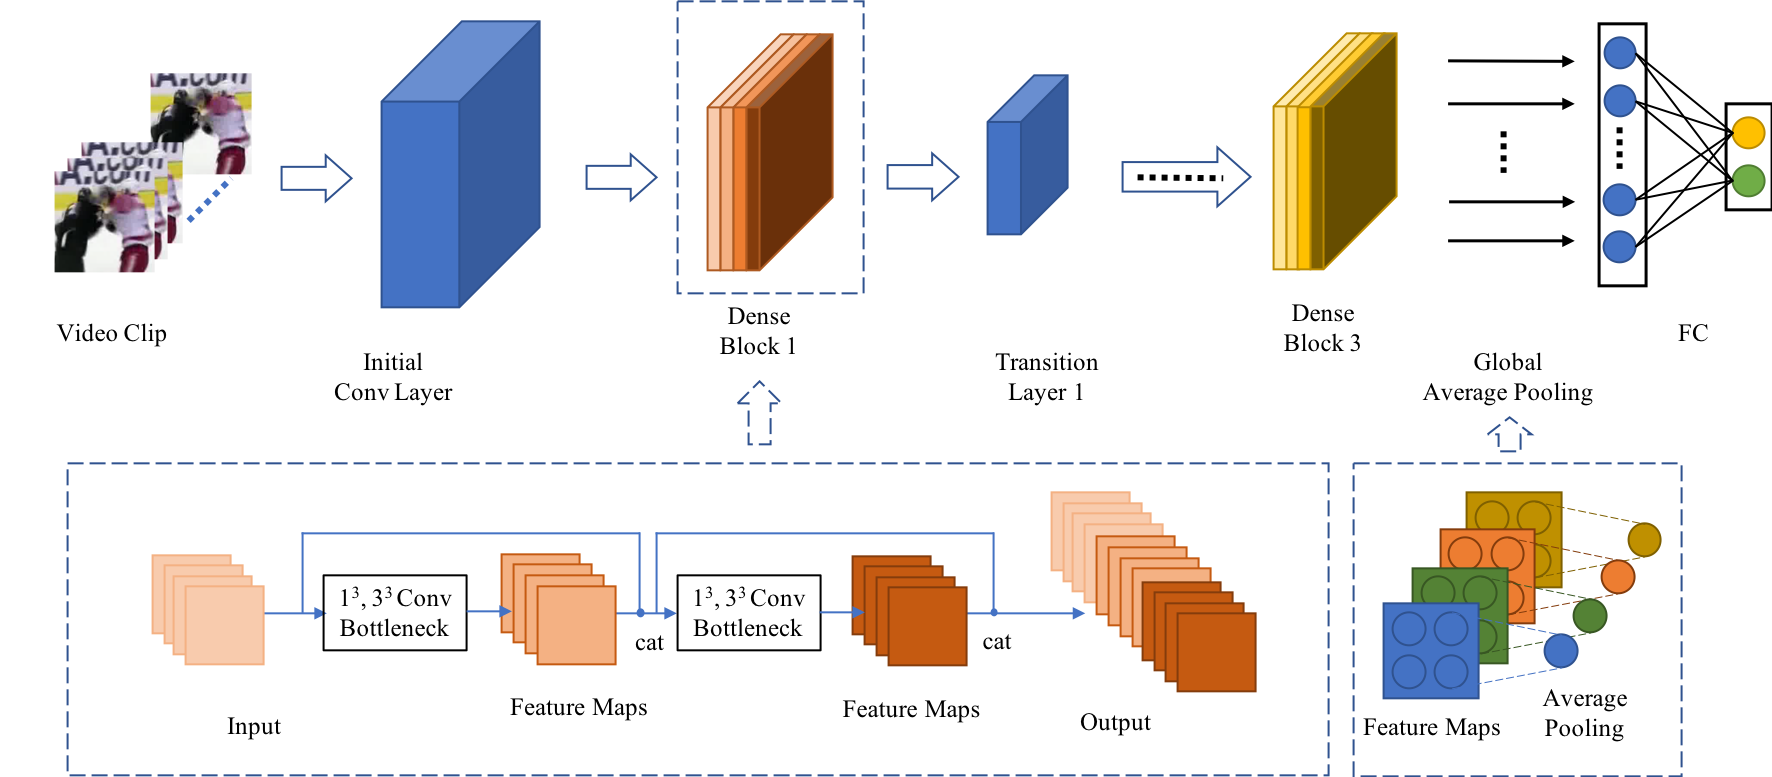
\includegraphics[scale=0.52]{fig/fig1.png}
\end{center}
\caption{Block diagram of the proposed model. This model is composed of an initial convolution layer, three dense blocks, two transition layers, and one fully connected layer. The figure omits Dense Block 2 and Transition Layer 2, due to the limitation of space. Each dense block contains several dense layers. The fully-connected layer is joined with output feature maps using global averaging pooling strategy.}
\label{fig:model}
\end{figure*}
	
	
%------------------------------------------------------------------------- 

\section{Proposed Method}
\label{sec:3}

The purpose of the proposed method is to design an end-to-end trainable deep learning model for detecting and recognizing fight clips in videos. 
For a model able to identify violent scenes, it should be capable of capturing anomaly or intense motions pattern of human bodies. 
Recognition accuracy and computational efficiency are two important indicators.
Consequently, developing effective and efficient spatiotemporal modules is of great importance in this task.
In view of the facts above, we leverage the findings in \cite{3dcnn_1, 3dcnn_2, r2+1d} and refer to the successful architecture of DenseNet \cite{densenet}, then finally develop a deep learning model based on 3D convolutional networks.

\subsection{Rethinking 3D Convolutional Networks}

For video understanding tasks, the most critical issue is how to extract appropriate features that are representative of the spatiotemporal information.
Compared to those architectures that separately encode spatial and temporal information, 3D CNNs can simultaneously capture spatiotemporal features as its convolution kernel extended to three dimensions. 
It implies that there is no need to apply extra LSTM or other RNN architectures exclusively designed for encoding temporal information. 
Also, raw pixels can be input directly without complicated preprocessing or extra calculation, which is much more computationally efficient than other deep learning model using optical flow, trajectories, and so forth.

However, the number of parameters may  exponentially increase as 3D convolution filters cube the kernel size, which may bring two main problems: 
Firstly, more parameters require higher FLOPs, which is computational inefficient; 
Secondly, redundant parameters may result in model overfitting and decreased generalization ability, especially in small scale datasets. 
To address these problems and promote 3D CNNs to give scope to its representation potentials, we have adopted several strategies.

The most direct method is to reduce the kernel size of convolution filters. 
For instance, two serialized 3$\times$3$\times$3 kernels have nearly the same representation ability of one 5$\times$5$\times$5 kernel, while the number of parameters is only half. 
Also, findings in \cite{3dcnn_1, 3dcnn_2, r2+1d} suggest that 3$\times$3$\times$3 kernel size is the best option for 3D CNNs.

Encouraging feature reusing is also a good practice in designing networks. 
In the model training phase, it helps to facilitate the backpropagation of information flow, which conduces to avoid overfitting and improve generalization. 
DenseNet \cite{densenet} gives serials of inspirations on developing compact but effective network architectures.

\subsection{Network Architecture}

An overview of the proposed model is illustrated in Figure \ref{fig:model}, including three dense blocks and two transition layers. 
All the kernel sizes of convolution filters and pooling layers are three-dimensional. 
The network takes video clips as inputs, from which the initial convolution layer produces first 64 feature maps. 
Then these feature maps are handled in the following first dense block. 
Dense block composes of several densely connected layers, namely dense layers.
The $l^{th}$ dense layer receives all the feature maps produced by its preceding layers, $y_0$, $y_1$, $\cdots$, $y_{l-1}$, as inputs:
\begin{equation}
\label{eq:densenet}
y_l = H_l\left([y_0, y_1, \cdots, y_{l-1}]\right)
\end{equation}
where $H_l(*)$ is the state transition function of the $l^{th}$ layer, and $[*]$ denotes concatenating operation.
Each dense layer produces $k$ new feature maps, where $k$ is a hyper-parameter called growth rate. 
For a dense block containing $L$ layers, it produces $k \times L$ new feature maps.
Diagram in the left dashed box of Figure \ref{fig:model} illustrates a simplified mechanism in the dense block, where the number of dense layers is 2 and the growth rate $k$ is 4.
It outputs 12 feature maps, 8 of which are newly produced by its dense layers.

At the end of this model, we adopt the global average pooling strategy proposed in \cite{NinN} to bridge the convolutional networks with a fully connected layer for classification.
As is illustrated in the right dashed box of Figure \ref{fig:model}, the final output feature maps ($T \times H \times W$ tensors) are separately pooled into scalars.
It is conducive to avoid overfitting and can improve the generalization ability of the model. 
Meanwhile, it is more parameter saving compared to direct connection, implying a better computational efficiency.

Violent or aggressive behaviors contain not only simple movement patterns but also abstract high-order features like acceleration, duration, and body interaction.  
By feature reusing, the collective knowledge in every stage of the model is preserved and utilized by the final classifier for the final judgment, or rather a fusion based on the diversified and composed features, which can achieve more robust and generalized model. 

%------------------------------------------------------------------------- 

\begin{figure}[t]
\begin{center}
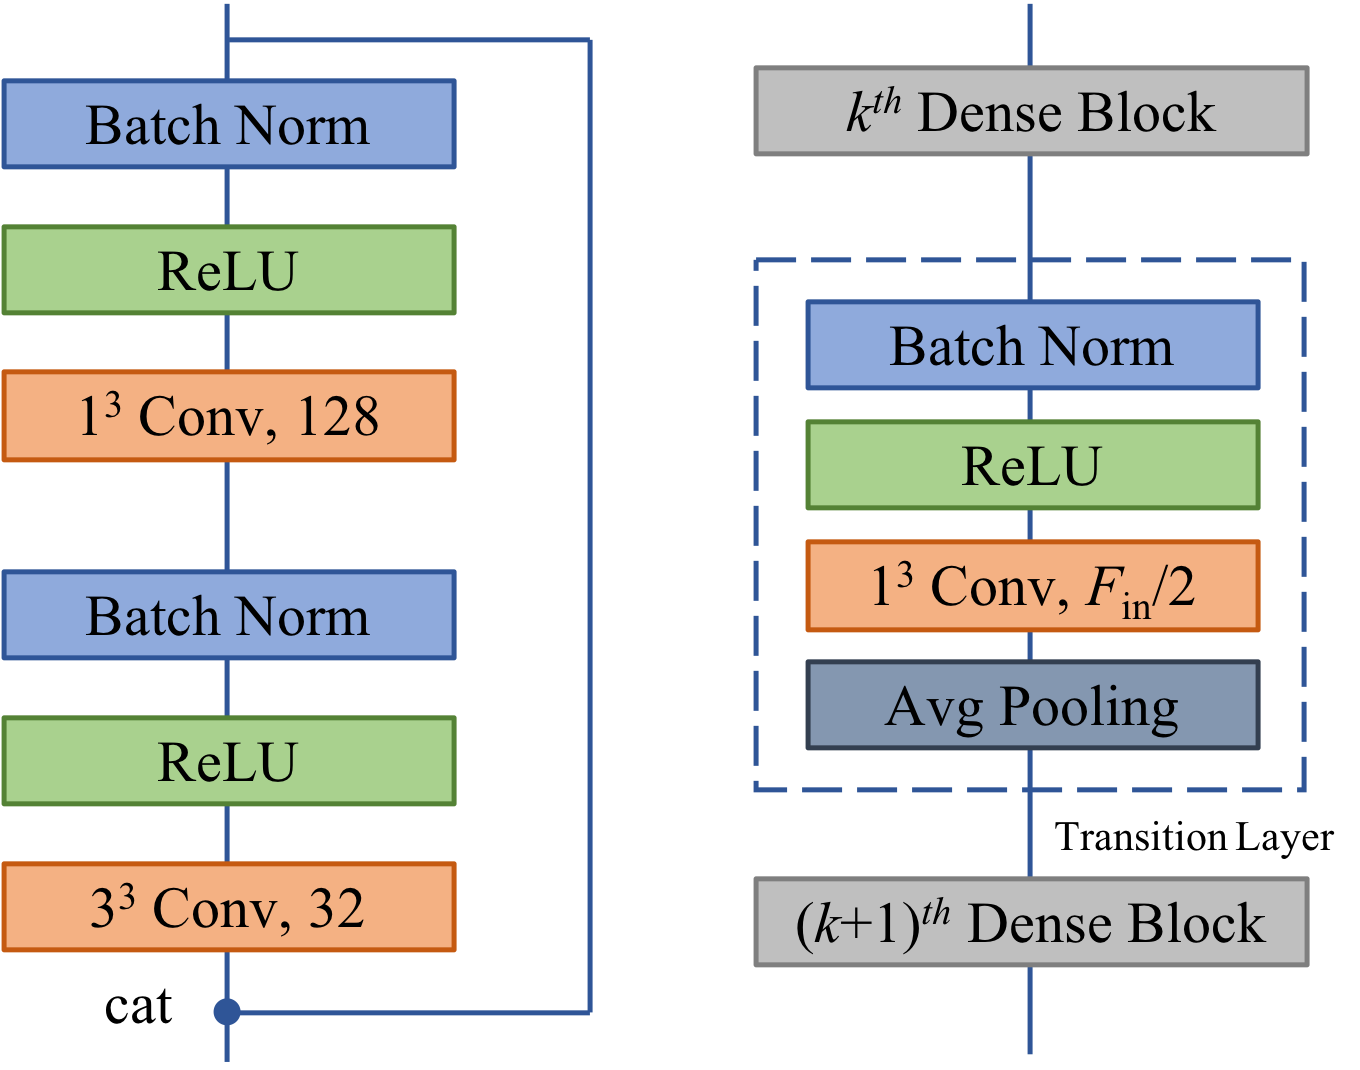
\includegraphics[scale=0.32]{fig/fig2.png}
\end{center}
\caption{Block diagram of bottleneck and transition layer. The block [$x^3$ Conv, $F$] denotes a convolution filter that has the kernel size of $x \times x \times x$ and produces $F$ feature maps.}
\label{fig:bottleneck}
\end{figure}

%------------------------------------------------------------------------- 

\subsection{Internal Details}

Dense layer should be elaborately designed since it is the basic unit for feature learning. 
Here, \emph{Bottleneck} architecture with pre-activation is adopted in every dense layer. 
The left diagram in Figure \ref{fig:bottleneck} represent the bottleneck architecture, whose growth rate is 32 and bottleneck size is 4.
The $1 \times 1 \times 1$ convolution layer produces $32 \times 4$ intermediate feature maps, followed by $3 \times 3 \times 3$ convolution layer that produces 32 (growth rate) output feature maps.
Typically, a dense layer on the later place has more inputs as it receives all the feature maps from its preceding layers. 
Consequently, using bottleneck helps to compact feature maps, thus improves computational efficiency.
Meantime, the expansion inside bottleneck promotes information interaction between different channels, which is favorable for learning complex features.

Transition layer is placed between any two dense blocks, as is illustrated in the right diagram of Figure \ref{fig:bottleneck}.
The objective of placing transition layer is to downsample feature maps and match the number of output and input feature maps between adjacent blocks.
Here we set the number of output feature maps equal to half of the input, as $F = F_{in}/2$.
In addition to reducing the complexity and tuning the nonlinearity of the model, the transition layer can also help to promote interaction between channels, which enhances the feature learning ability and improves the robustness of our model.

Table \ref{table:arch} lists the details of the proposed model.
In the column of output shape, $[F, T, H, W]$ denotes the shape of tensors (feature maps) produced by the corresponding module.
Note that dense blocks are slightly different from the simplified illustration in Figure \ref{fig:model} as they use the bottleneck in Figure \ref{fig:bottleneck}. 

%------------------------------------------------------------------------ 

\begin{table}[t]
\begin{center}
\caption{Network architecture of the proposed model.}
\label{table:arch}
\begin{tabular}{lcr}
\hline
\textbf{Module Name} & \textbf{Architecture} & \textbf{Output Shape} \\
\hline\hline
Input Clip & - & [3,16,112,112] \\
Initial Conv & $7^3$ Conv, (1,2,2) & [64,16,56,56] \\
Pooling & $3^3$ Max & [64,8,28,28] \\
DenseBlock 1 & $(1^3, 3^3) \times 6$ & [256,8,28,28] \\
TransitionLayer 1 & $1^3$ Conv, $3^3$ Avg & [128,4,14,14]\\
DenseBlock 2 & $(1^3, 3^3) \times 12$ & [512,4,14,14] \\
TransitionLayer 2 & $1^3$ Conv, $3^3$ Avg & [256,2,7,7] \\
DenseBlock 3 & $(1^3, 3^3) \times 24$ & [1024,2,7,7]\\
GlobalAvgPooling & $2 \times 7 \times 7$ Avg & [1024,1,1,1]\\
Classification & FC Layer & [2, -, -, -] \\
\hline
\end{tabular}
\end{center}
\footnotesize
For $3^3$ convolution and pooling, the default stride is (2,2,2). The $(1^3, 3^3)$ denotes the bottleneck architecture in Figure \ref{fig:bottleneck}.
\end{table}

%------------------------------------------------------------------------ 

\begin{table*}[t]
\begin{center}
\caption{Comparison of classification accuracy on three standard datasets.}
\label{table:result}
\begin{tabular}{lccc}
\hline
\textbf{Method} & \textbf{Hockey Fights Dataset} & \textbf{Movies Dataset} & \textbf{VIolent Flows Dataset} \\
\hline\hline
ViF + OViF \cite{ovif} & 87.5$\pm$1.7\% & - & 88$\pm$2.45\% \\
Radon Transform \cite{fast} & 90.1$\pm$0\% & 98.9$\pm$0.22\% & - \\
STIFV \cite{bilinski2016human} & 93.4\% & 99\% & 96.4\% \\
MoIWLD \cite{MoIWLD} & 96.8$\pm$1.04\% & - & 93.19$\pm$0.12\% \\
OR-VLAD \cite{vlad} & 98.2$\pm$0.76\% & \textbf{100$\pm$0\%} & 93.09$\pm$1.14\% \\
\hline
Three streams + LSTM \cite{dong2016multi} & 93.9\% & - & - \\
FightNet \cite{zhou2017violent} & 97.0\% & 100\% & - \\
Hough Forests + CNN \cite{serrano2018fight} & 94.6$\pm$0.6\% & 99$\pm$0.5\% & - \\
ConvLSTM \cite{convlstm_sudh} & 97.1$\pm$0.55\% & \textbf{100$\pm$0\%} & 94.57$\pm$2.34\% \\
Bi-ConvLSTM \cite{bi_convlstm} & 98.1$\pm$0.58\% & \textbf{100$\pm$0\%} & 93.87$\pm$2.58\% \\
\textbf{Proposed} & \textbf{98.3$\pm$0.81\%} & \textbf{100$\pm$0\%} & \textbf{97.17$\pm$0.95\%} \\
\hline
\end{tabular}
\end{center}
\end{table*}

%------------------------------------------------------------------------ 

\section{Experiments and Analyses}
\label{sec:4}

An experiment has been conducted to validate the performance of the proposed model on three standard benchmark datasets.
Meanwhile, in the supplementary experiments, effectiveness and efficiency are also evaluated.

\subsection{Dataset}

In violence detection tasks, there are three public benchmark datasets: \\
\textbf{Hockey Fights Dataset} \cite{hockey} contains 1000 videos collected from hockey games.
Each video consists of 50 frames of 720$\times$576. 
All videos have the same background and similar human activities, including fights and normal gaming. \\
\textbf{Movies Dataset} \cite{hockey} has 200 video clips fetched from action movies with different resolutions. Slightly different from Hockey, videos in Movies dataset vary in contents.\\
\textbf{VIolent-Flows Dataset} \cite{vif} consists of 246 videos of crowd behavior with frames resized to 320$\times$240 pixels.
Multiple perspectives, noisy background, and dense crowd make this dataset challenging compared to the other two.

All of these three datasets contain balanced fight and non-fight videos. 
However, as designed for hand-crafted methods, these datasets are relatively small in scale, which may not be capable of training deep neural networks.
To cope with this problem, ConvLSTM \cite{convlstm_sudh} adopting AlexNet model pre-trained on ImageNet.
Similarly, we consult the findings in \cite{3dcnn_2} and utilize partial parameters of their model, which is pre-trained on Kinetics dataset \cite{kinetics}.
These parameters are imported to initialize the initial convolution layer in our model.

These three datasets are also combined as Mix dataset.
In Mix dataset, positive and negative samples are randomly drawn from original datasets separately in the same proportion.
Mix dataset can be used to evaluate overall performance for deep learning models of their modeling capability and generalization ability in violence detection tasks.

\subsection{Experiment Setup}

The proposed model is implemented using PyTorch \cite{pytorch} platform. 
Deep models for comparison on effectiveness and efficiency are also implemented using PyTorch to guarantee comparability and consistency.

Network inputs are prepared as tensors with shape $N \times C \times T \times H \times W$, in which $N$ is the batch size, $C$ is the number of channels (3 for RGB videos), $T$ is the duration of clips and $H \times W$ denotes the frame resolution. 
In the experiment, each video is sampled with 16 adjacent frames and then cropped and resized into 112$\times$112 pixels.

In the training phase, data augmentation is employed to enlarge training set and reduce overfitting, including random horizontal flipping, spatially random scale cropping, and temporally random slicing. 
The learning rate and batch size are $10^{-3}$ and $32$ for Hockey and $10^{-4}$ and $16$ for Movie and ViF, considering the scales of datasets.
We apply mini-batch stochastic gradient descent (SGD) with momentum 0.5 and weight decay $10^{-3}$ for model optimization.  
Cross entropy function defined in \ref{eq:crossentropy} is used for loss calculation. 
\begin{equation}
\label{eq:crossentropy}
\operatorname{loss}(x, \text{label}) = -\log \left(\frac{\exp (x[\text{label}])}{\sum_{j} \exp (x[j])}\right)
\end{equation}

In the evaluation phase, videos in test set are spatially cropped around center pixels and temporally sliced to use center adjacent frames.
Other boosting strategies like sliding window, resampling, and voting are not adopted, in order to validate the baseline performance of the proposed model.

For the supplementary experiment on Mix dataset, we split 1,446 videos into training and validation set with 9:1. 
The ConvLSTM \cite{convlstm_sudh} model is optimized using RMSprop algorithm, while other models are still trained by SGD algorithm with momentum.
The batch size and learning rate are set to 32 and $10^{-3}$.

\subsection{Results and Analyses}

\noindent\textbf{Experiment on Standard Datasets}

In this experiment, we adopt five-fold cross validation to evaluate the recognition performance of the proposed model.
Table \ref{table:result} gives the classification accuracy of the state-of-the-art methods on three standard datasets.
The top half of the table lists hand-crafted methods, with deep learning models listed in the bottom half.
From this table, it can be concluded that deep learning methods generally perform better than hand-crafted methods.
Among all of them, the proposed model achieves the best performance on all of these three datasets.

As explained in Section \ref{sec:1}, violence is considered as aggressive behaviors of human. 
Consequently, it may be obscure to distinguish fights from other human body movements like sports and celebrations.
For instance, in Hockey Fights dataset, regular games also involve physical collisions and intense movements, which is confusing and has a real possibility to be mistaken as violence.
Nevertheless, the proposed model achieves the highest accuracy, indicating that it is capable of capturing effective spatiotemporal features and high order localized region information.

In Movies dataset, there are identifiable differences between positive and negative samples in contents.
As a result, all models perform well.

However, in VIolent-Flows dataset, dense crowd and noisy background make it challenging for feature learning.
Multi-scale and multi-viewpoint may also interfere with the effectiveness of models as motion patterns vary from different perspectives.
In this case, nevertheless, the proposed model achieves the highest accuracy and relatively low variance.
Owing to the design of feature reusing and channel interaction, the proposed model can form the mechanism of multi-attentions for discovering specific regions and capturing anomaly motion patterns in videos.
Also, global average pooling before classification provides global fields of features that are more robust for the final decision.

%------------------------------------------------------------------------ 

\begin{table}[t]
\begin{center}
\caption{Experiment results on Mix dataset.}
\label{table:mix}
\begin{tabular}{lccc}
\hline
\textbf{Model} & \textbf{Accuracy} & \textbf{CE Loss} & \textbf{\# Params} \\
\hline\hline
C3D \cite{3dcnn_1} & 92.47\% & 0.4019 & 78.0M \\
ConvLSTM \cite{convlstm_sudh} & 96.58\% & 0.1355 & 9.6M \\
\textbf{Proposed} & \textbf{99.32\%} & \textbf{0.0326} & \textbf{7.4M} \\
\hline
\end{tabular}
\end{center}
\end{table}

\begin{figure}[t]
\begin{center}
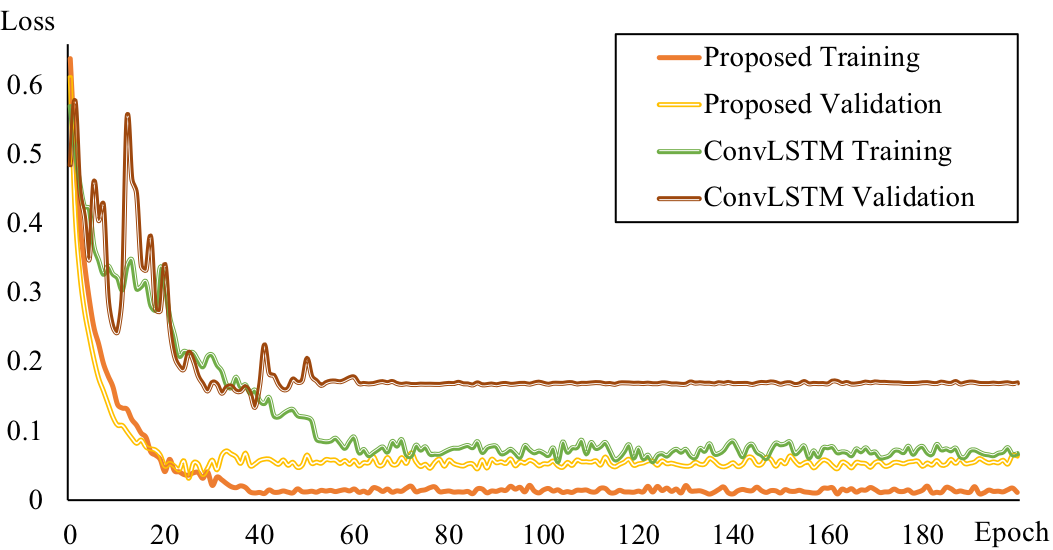
\includegraphics[scale=0.46]{fig/fig3.png}
\end{center}
\caption{Training and validation losses of the proposed model and ConvLSTM \cite{convlstm_sudh} on Mix dataset.}
\label{fig:mix}
\end{figure}

%------------------------------------------------------------------------

\noindent\textbf{Experiment on Mix Dataset}

Supplementary experiment on Mix dataset is carried out to evaluate the effectiveness of deep learning models.
The proposed model is compared with two representative models, C3D and ConvLSTM.
C3D \cite{3dcnn_1} is a classic video discriptor based on 3D CNNs, and ConvLSTM \cite{convlstm_sudh} is one of the state-of-the-art models in violence detection tasks.

Table \ref{table:mix} compares the effectiveness and parameter numbers of these models.
Among them, the proposed model has a higher classification accuracy with relatively fewer parameters.
The cross entropy loss of our model on validation set is 0.0326, an order of magnitude lower than 0.1355 of ConvLSTM.
Compared to C3D model, the proposed model saves up to 90\% parameters, but can more effectively learn the representations thanks to the narrow bottleneck architectures and global average pooling strategy.

Figure \ref{fig:mix} illustrates the losses in training and validation epochs for the proposed model and ConvLSTM.
The learning curves of the proposed model are smoother and faster in convergence, and finally, level out at relatively lower losses.
It implies that our model is more capable of learning abstract features and modeling motion patterns, which helps to achieve better generalization ability.
However, the slight rebound in validation curves of both models indicates the minor overfitting, maybe the scale of existing datasets is still insufficient for training deep networks. 

\noindent\textbf{Evaluation on Efficiency}

The efficiency of models is theoretically studied and practically estimated using torch.autograd.profiler library on single GTX 1080Ti.
Table \ref{table:efficiency} shows that the proposed model requires lower floating point operations (FLOPS), which needs less computing resources and can work more efficiently.
It has a faster inference speed and can process about 175 16-channel frames per second.
However, limitations are that our model demands frequent memory read-write operations, due to the implementation of feature reusing, resulting in inferior performance on small batch input.
It may cost more time on some low-end devices.
We will try to optimize its implementation and fix this problem.

%------------------------------------------------------------------------ 

\begin{table}
\begin{center}
\caption{Quantized performance of efficiency.}
\label{table:efficiency}
\begin{tabular}{lcccc}
\hline
\textbf{Model} & \textbf{FLOPS} & \textbf{1} & \textbf{8} & \textbf{16}\\
\hline\hline
C3D \cite{3dcnn_1} & 40.04G & \textbf{1.1ms} & 5.1ms & 9.9ms \\
ConvLSTM \cite{convlstm_sudh} & 14.40G & 3.7ms & 4.9ms & 6.3ms \\
\textbf{Proposed} & \textbf{10.43G} & 1.9ms & \textbf{3.6ms} & \textbf{5.7ms} \\
\hline
\end{tabular}
\end{center}
\footnotesize
The last three columns list the $n$-channel (i.e., input with $n$ batches) inference latency per frame on single GTX 1080Ti.
\end{table}

%------------------------------------------------------------------------

\section{Conclusions}
\label{sec:5}

In this paper, we propose a deep learning model based on 3D convolutional neural networks with improved internal architecture. 
The proposed model has relatively fewer parameters and can effectively learn spatiotemporal features of violent behaviors. 
Experiment results on three standard benchmark datasets demonstrate the improvements of our model over methods. 
Also, the supplementary experiment on Mix dataset proves the effectiveness of our model on representation learning. 
At last, we evaluate the efficiency of deep learning models from theoretical and practical aspects.
The proposed model is computing resource-saving, very efficient, and capable of real-time processing. 

For practical applications, strategies such as sliding window and voting can be adopted to achieve better recognition accuracies. 
By selecting appropriate sample rates, it is feasible to make trade-offs between efficiency and accuracy for violence detection tasks in various scenarios.

{\small
\bibliographystyle{ieee}
\bibliography{egbib}
}

\end{document}
